
\chapter{Preliminaries} \label{chap:preliminaries}

\section{Computational models and Turing machines}

Throughout history, humans have been solving problems through a wide variety of models capable of computing valid results, ranging from their intellect to mechanical devices capable of solving problems. In particular, each computational model can be described as a list of sequential operations. Given the same initial conditions, these lists are expected to yield the same exact result each time the computation is executed.

In modern mathematics, this is described through the concept of \textbf{algorithm}, which is a finite list of unambiguous instructions that, given some set of initial conditions, can be performed to compute the answer to a given problem. Even though this is a straightforward definition for an algorithm, it isn't as "mathematically stable" as it seems: each computational model could have access to a different set of possible operations, meaning that the same problem could be solved by different kinds of algorithms. In 1950, Alan Turing was able to define a theoretical computational model capable of capturing the concept of computation itself through a simple - but sufficient - theoretical machine, i.e. the now called \textbf{Turing machine}.  \cite{complexity_arora_barak, sipser_computation}

A Turing machine is made of:
\begin{itemize}
    \item A \textit{tape} divided into cells, where each cell contains a symbol from a finite set called \textit{alphabet}, usually assumed to contain only 0 and 1, or a special symbol $\blankchar$, namely the \textit{blank character}. The tape is finite on the left side but infinite on the right side. 
    \item A \textit{read-write head} capable of reading and writing symbols on the tape. The head is always positioned on a single cell of the tape and can shift left and right only one cell per shift.
    \item A finite set of \textit{states} that can be assumed by the machine. At all times the machine only knows its current state. The set contains at least one state that is capable of immediately halting the machine when reached (such states could be unreachable, making the machine go in an infinite loop).
    \item A finite set of \textit{instructions} which, given the current state and the current cell read by the read-write head, dictate how the machine behaves. Each instruction tells the machine to do three things: replace the symbol of the current cell (which can be replaced with itself), move the head one cell to the left or one cell to the right and move from the current state to a new one (which can be the current state itself).
\end{itemize}

Initially, the machine's tape contains only an \textit{input string}, while all the other infinite cells contain the blank character. At the end of the computation, the tape contains only the \textit{output string}, which is the result of the computation.

\begin{figure}[H]
    \centering
    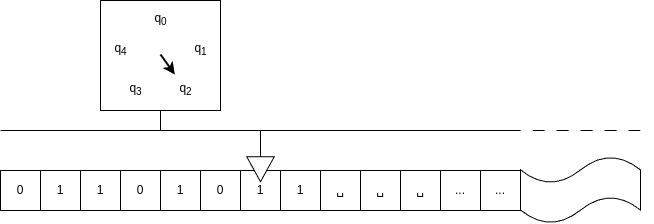
\includegraphics[scale=0.5]{resources/images/tm.png}

    \caption{A Turing Machine}
\end{figure}

The \textit{Church-Turing thesis} states that it suffices to restrict attention to this single model since it can compute all computable mathematical functions with only a little loss of efficiency. This result can characterize the concept of algorithm through Turing machines themselves. \cite{complexity_arora_barak}

\begin{definition}
 A Turing machine is a 7-uple $M = (Q, F, \Gamma, \Sigma, q_0, \delta)$ where:
    \begin{itemize}
        \item $Q$ is a finite set of states, $F \subseteq Q$ is a finite set of halting states and $q_0 \in Q$ is the initial state taken by the machine.
        \item $\Gamma$ is a finite set of symbols, usually called the tape alphabet. The tape alphabet always contains the symbol $\blankchar\,$.
        \item $\Sigma$ is a finite set of symbols, usually called the input alphabet, where $\Sigma \subseteq \Gamma - \{\blankchar\}$. The input string can be formed only of these characters.
        \item $\delta : (Q - F) \times \Gamma \to Q \times \Gamma \times \{\mathsf{L}, \mathsf{R}\}$ is a partial function, usually called the transition function, where $\mathsf{L}$ and $\mathsf{R}$ represents a left or right shift of the read-write head. Intuitively, if $\delta(q, a) = (p, b, L)$ then when the machine is in state $q$ and reads the symbol $a$ on the current cell of the tape then it transitions to the state $p$, replaces the symbol $a$ with $b$ and moves the head to the left.
    \end{itemize}
\end{definition}

Turing proved the existence of an \textit{universal Turing machine}, a \TM that is capable of simulating any other Turing machine. This result shouldn't be a surprise: modern computers are nothing more than universal \textsf{TM}s that can execute any given algorithm. A generic computational model is said to be \textit{Turing complete} when it can simulate a universal Turing machine. In other words, a Turing complete computational model is capable of performing every possible computation.

\newpage

\section{Complexity measures}

After being able to give a mathematically stable definition of computation through Turing machines, researchers shifted their focus to understanding which problems are computable. In particular, they showed that some problems are \textbf{uncomputable} by proving that there cannot exist a Turing machine capable of carrying out their computation without going in infinite loops and never halting, such as Turing's famous \textit{Halting problem}, i.e. determining if a machine will halt or not for a given input.

A "good" algorithm (or \TM) should be able to solve the associated problem in an efficient way. But what does it mean for a \TM to be \textit{efficient}? To formally define this idea, computer scientists defined \textbf{complexity measures} to quantify the amount of computational resources needed by a Turing machine. An efficient \TM should be able to solve a task with low computational resources. Above all, we are interested in studying the amount of steps needed and the amount of cells needed to achieve such computations. These two concepts are referred to as the \textit{time complexity} and the \textit{space complexity} of a Turing machine.

\begin{definition}
 Given a Turing machine $M$, we define the time complexity and space complexity of $M$ as the two functions $t, s : \N \to \R^+$ such that $t(n)$ and $s(n)$ are respectively the maximum number of steps and initially blank cells used by $M$ to compute an input string of length $n$.
\end{definition}

Time and space complexity are intrinsically related one to the other: time limits the amount of space and vice versa. Usually, these two measures are proportionally inverse: if we allow our algorithm to use more space then the computation can be sped up, while if we want a low amount of used space then the computation will require more steps. These reasons are enough to make both time and space an interesting measure to evaluate the efficiency of an algorithm.

Usually, larger inputs require a larger amount of computational resources, making the values $t(n)$ and $s(n)$ proportional to the size $n$ of the input. For this reason, as the input size grows, we are interested in the asymptotic behavior of these measures. This concept is captured by the so-called \textit{big-Oh notation}.

\begin{definition}
 Given two functions $f, g : \N \to \R^+$, we say that:
    \begin{enumerate}
        \item $f$ is in big-Oh of $g$, written as $f(n) = O(g(n))$, if there are two values $c, N \in \N_{> 0}$ such that $\forall n \geq N$ it holds that $f(n) \leq c g(n)$.
        \item $f$ is in Omega of $g$, written as $f(n) = \Omega(g(n))$, if there are two values $c, N \in \N_{> 0}$ such that $\forall n \geq N$ it holds that $f(n) \geq c g(n)$.
        \item $f$ is in Theta of $g$, written as $f(n) = \Theta(g(n))$, if there are three values $c,d, N \in \N_{> 0}$ such that $\forall n \geq N$ it holds that $c g(n) \leq f(n) \leq d g(n)$.
    \end{enumerate}
\end{definition}

\newpage

In other words, as the input size $n$ grows the function $f$ can dominate, be dominated or both by a function $g$, defining the \textit{lower} and \textit{upper} bounds of the value $f(n)$. In particular, when $f(n) = \Theta(g(n))$ the two functions can be considered to be \textit{almost} the same due to them following the same growth pattern. Additionally, its easy to see that $f(n) = \Omega(g(n))$ if and only if $g(n) = O(f(n))$ and likewise that $f(n) = \Theta(g(n))$ if and only if $f(n) = O(g(n))$ and $f(n) = \Omega(g(n))$. 

Efficiency dictates whether a problem is actually feasible or not in the real world: if a problem is computable by a \TM but requires an immense amount of time or space to get to the result, then the computation is practically unachievable. These problems are often referred to as \textbf{intractable problems} \cite{complexity_arora_barak,sipser_computation}.

Complexity is generally measured in terms of asymptotic behavior. An algorithm is considered time efficient if it can compute the answer in at most a polynomial amount of time, i.e. in $O(n^k)$ time for some $k \in \N$. Likewise, it is considered space efficient if it can compute the answer in at most a logarithmic amount of space, i.e. in $O(\log^k n)$ space for some $k \in \N$.

For example, consider the following informally defined Turing machine $M$ which takes the binary encoding $\abk{m}$ of a natural number $m \in \N$ as the input string and returns $\abk{m^2}$ as the output string. The computation made by $M$ is achieved by repeatedly adding the value $m$.

$M$ = "Given the input string $\abk{m}$:
    \begin{enumerate}
        \item Copy the string $\abk{m}$ on a blank set of contiguous cells. This copied string will be referred to as the value $k$.
        \item Copy the string $\abk{m}$ on a blank set of contiguous cells. This copied string will be referred to as the value $y$.
        \item Repeat while the value $k$ is bigger than $1$:
        \begin{enumerate}[label={\arabic*.}, start=3]
            \item Copy the string $\abk{y}$ on a blank set of contiguous cells. This copied string will be referred to as the value $x$.
            \item Compute $x + n$ and store the result on the space occupied by the string $\abk{y}$. In other words, compute $y \gets x + n$.
            \item Compute $k - 1$ and store the result on the space occupied by the string $\abk{k}$. In other words, compute $k \gets k - 1$.
        \end{enumerate}
    \end{enumerate}
    \begin{enumerate}[label={\arabic*.}, start=6]
        \item Write $\blankchar$ on all the cells on the tape, except for the cells of the string $\abk{o}$.
        \item Halt the machine and return the output string $\abk{o}$."
    \end{enumerate}

 We know that any natural number $m \in \N$ can be encoded in binary with $\log_2 m$ bits. This means that the length $n$ of the input string $\abk{m}$ is $\log_2 m$.
    
 Consider now the values $k$ and $o$ obtained in the computation. These values are natural numbers and they can clearly be expressed as a real multiple of the value $m$. This means that $k, x, y = O(m)$ and thus they can be encoded with $O(\log m)$ bits (asymptotic notation allows us to drop the subscript of the logarithm), thus our requiring $3 \cdot O(\log m)$ cells, which is asymptotically equivalent to $O(\log m)$ cells. We conclude that the space complexity of such $\TM$ is $O(\log m) = O(n)$.

 To copy a string of length $\ell$, the Turing machine needs to copy $\ell$ cells but also requires to make additional shifts in order to repeatedly move from the original string to the copied one, making the total amount of steps required $O(\ell)$. In a similar fashion, binary addition (or subtraction) between two numbers $a$ and $b$ can be computed in $O(\log a + \log b)$ steps. Since we initially set $k = m$ and the machine decrements the value of $k$ by 1 on each iteration of the loop, the computations inside the loop get executed $m-1$ times. This means that the total number of steps of the loop is $O((m-1) \log m)$. By adding the initial two copy procedures, the total number of steps done by the machine is $O(2 \log m + (m-1) \log m)$, which is asymptotically equivalent to $O(m \log m)$ cells. Thus, we conclude that the time complexity of such $\TM$ is $O(m \log m) = O(2^n n)$.
    
 This implies that the example algorithm defined above is inefficient in both time and space, making repeated addition one of the worst ways to solve this task. But does this mean that the problem is intractable? Modern computers can square a number in milliseconds, so the answer to this question should clearly be no. In fact, even by implementing the column method for multiplying numbers usually taught to kids we could solve the problem in a very low amount of steps but a not-so-efficient amount of space.

    
 Efficiency is the lingering question that torments modern computer scientists. We know that some problems are computationally unattainable, but where is the line that separates tractable and intractable problems? What property defines problems that cannot be solved efficiently? Finding an answer to these questions may seem easy, but, even after more than 70 years of research, the question persists in the mind of complexity theorists.

\cleardoublepage